\begin{center}
	\begin{tabular}{M{9.25cm}M{8.75cm}}
		\textbf{TRƯỜNG THCS-THPT NGUYỄN KHUYẾN}& \textbf{ÔN TẬP KTTX LẦN 2 - HỌC KÌ II}\\
		\textbf{MÃ ĐỀ: 001}& \textbf{Bài thi môn: VẬT LÝ 10}\\
		\textit{(Đề thi có 04 trang)}& \textit{Thời gian làm bài: 45 phút, không kể phát đề}
		
		\noindent\rule{4cm}{0.8pt} \\
	\end{tabular}
\end{center}
\begin{center}
	\textit{Lấy gia tốc rơi tự do $g=\SI{10}{\meter/\second^2}$; khối lượng riêng của nước $\rho=\SI{1000}{\kilogram/\meter^3}$; $\SI{1}{HP}=\SI{746}{\watt}$.}
\end{center}
\setcounter{section}{0}
\section{Câu trắc nghiệm nhiều phương án lựa chọn}
\textit{Thí sinh trả lời từ câu 1 đến câu 12. Mỗi câu hỏi thí sinh chọn một phương án}
\setcounter{ex}{0}
\Opensolutionfile{ans}[ans/D10-KTTX2-HK2-TN]
% ===================================================================
\begin{ex}
	Công suất được xác định bằng
	\choice
	{\True công thực hiện trong một đơn vị thời gian}
	{công thực hiện trong đơn vị dài}
	{tích của công và thời gian thực hiện công}
	{tổng độ lớn công phát động}
	\loigiai{}
\end{ex}
% ===================================================================
\begin{ex}
	Một quả bóng được ném tung lên cao từ mặt đất, sau đó rơi trở lại đất. Công của trọng lực trong suốt quá trình này bằng
	\choice
	{$mgh$}
	{\True $0$}
	{$2mgh$}
	{không xác định được}
	\loigiai{}
\end{ex}
% ===================================================================
\begin{ex}
	Một ô tô đang chạy trên đường với tốc độ \SI{72}{\kilo\meter/\hour}. Công suất của động cơ là \SI{60}{\kilo\watt}. Lực phát động của động cơ là
	\choice
	{\SI{2500}{\newton}}
	{\True \SI{3000}{\newton}}
	{\SI{2800}{\newton}}
	{\SI{1550}{\newton}}
	\loigiai{}
\end{ex}
% ===================================================================
\begin{ex}
Một vật có khối lượng $m=\SI{100}{\gram}$ trượt xuống mặt phẳng nghiêng dài \SI{3}{\meter} và nghiêng \SI{30}{\degree} so với phương ngang. Công của trọng lực tác dụng lên vật là
	\choice
	{\True \SI{1.5}{\joule}}
	{\SI{-1.5}{\joule}}
	{\SI{3}{\joule}}
	{\SI{-3}{\joule}}
	\loigiai{}
\end{ex}
% ===================================================================
\begin{ex}
	Một máy bơm nước mỗi giây có thể bơm \SI{15}{\liter} nước lên bể nước ở độ cao \SI{10}{\meter}. Nếu coi tổn hao là không đáng kể. Công suất của máy bơm là
	\choice
	{\SI{150}{\watt}}
	{\SI{3000}{\watt}}
	{\True \SI{1500}{\watt}}
	{\SI{2000}{\watt}}
	\loigiai{}
\end{ex}
% ===================================================================
\begin{ex}
	Một lực kéo \SI{2500}{\newton} theo phương ngang tác dụng lên một chiếc xe khối lượng \SI{500}{\kilogram} đang đứng yên trên mặt đường nằm ngang. Biết tổng lực cản tác dụng lên xe có độ lớn \SI{1000}{\newton}. Công của lực kéo tác dụng lên xe khi xe chuyển động được \SI{2}{\second} là 
	\choice
	{\SI{6}{\kilo\joule}}
	{\SI{9}{\kilo\joule}}
	{\True \SI{15}{\kilo\joule}}
	{\SI{21}{\kilo\joule}}
	\loigiai{}
\end{ex}
% ===================================================================
\begin{ex}
	Một dây cáp sử dụng động cơ điện tạo ra một lực không đổi \SI{50}{\newton} tác dụng lên vật và kéo vật đi một đoạn đường \SI{30}{\meter} trong thời gian \SI{1}{\minute}. Công suất của động cơ là
	\choice
	{\SI{50}{\watt}}
	{\True \SI{25}{\watt}}
	{\SI{100}{\watt}}
	{\SI{75}{\watt}}
	\loigiai{}
\end{ex}
% ===================================================================
\begin{ex}
	Một động cơ điện được thiết kế để kéo thùng than nặng \SI{400}{\kilogram} từ dưới mỏ có độ sâu \SI{200}{\meter} lên mặt đất trong thời gian \SI{2}{\minute}. Hiệu suất của động cơ là \SI{80}{\percent}. Công suất toàn phần của động cơ là
	\choice
	{\True \SI{8.3}{\kilo\watt}}
	{\SI{6.6}{\kilo\watt}}
	{\SI{83}{\kilo\watt}}
	{\SI{66}{\kilo\watt}}
	\loigiai{}
\end{ex}
% ===================================================================
\begin{ex}
	Một động cơ có công suất tiêu thụ bằng $\SI{5}{\kilo\watt}$ kéo một vật có trọng lượng $\SI{12}{\kilo\newton}$ lên cao $\SI{30}{\meter}$ theo phương thẳng đứng trong thời gian $\SI{90}{\second}$ với vận tốc không đổi. Hiệu suất của động cơ bằng
	\choice
	{$\SI{100}{\percent}$}
	{\True $\SI{80}{\percent}$}
	{$\SI{60}{\percent}$}
	{$\SI{40}{\percent}$}
	\loigiai{Công cần thiết để kéo vật nặng lên cao $\SI{30}{\meter}$:
		$$A_i=Ph=\SI{360}{\kilo\joule}$$
		Công suất có ích để kéo vật:
		$$\calP_i=\dfrac{A_i}{t}=\SI{40}{\kilo\watt}$$
		Hiệu suất động cơ:
		$$H=\dfrac{\calP_i}{\calP_{tp}}\cdot\SI{100}{\percent}=\SI{80}{\percent}.$$}
\end{ex}
\Closesolutionfile{ans}
\section{Câu trắc nghiệm đúng/sai} 
\textit{Thí sinh trả lời từ câu 1 đến câu 4. Trong mỗi ý \textbf{a)}, \textbf{b)}, \textbf{c)}, \textbf{d)} ở mỗi câu, thí sinh chọn đúng hoặc sai}
\setcounter{ex}{0}\\
\Opensolutionfile{ans}[ans/D10-KTTX2-HK2-TF]
% ===================================================================
\begin{ex}
	Trong các phát biểu sau, phát biểu nào đúng, phát biểu nào sai?
	\choiceTF
	{Một vật đứng yên thì không thể mang năng lượng}
	{\True Có thể chuyển hóa năng lượng bằng cách thực hiện công}
	{Năng lượng là đại lượng vector}
	{\True Năng lượng có thể chuyển hóa từ dạng này sang dạng khác}
	\loigiai{}
\end{ex}
% ===================================================================
\begin{ex}
	Cùng đưa một khối vật liệu nặng \SI{50}{\kilogram} lên độ cao \SI{10}{\meter}, người kéo mất \SI{50}{\second} (Hình a), trong khi máy tời điện kéo chỉ mất \SI{10}{\second} (Hình b). Bỏ qua lực ma sát giữa dây và ròng rọc.
	\begin{center}
		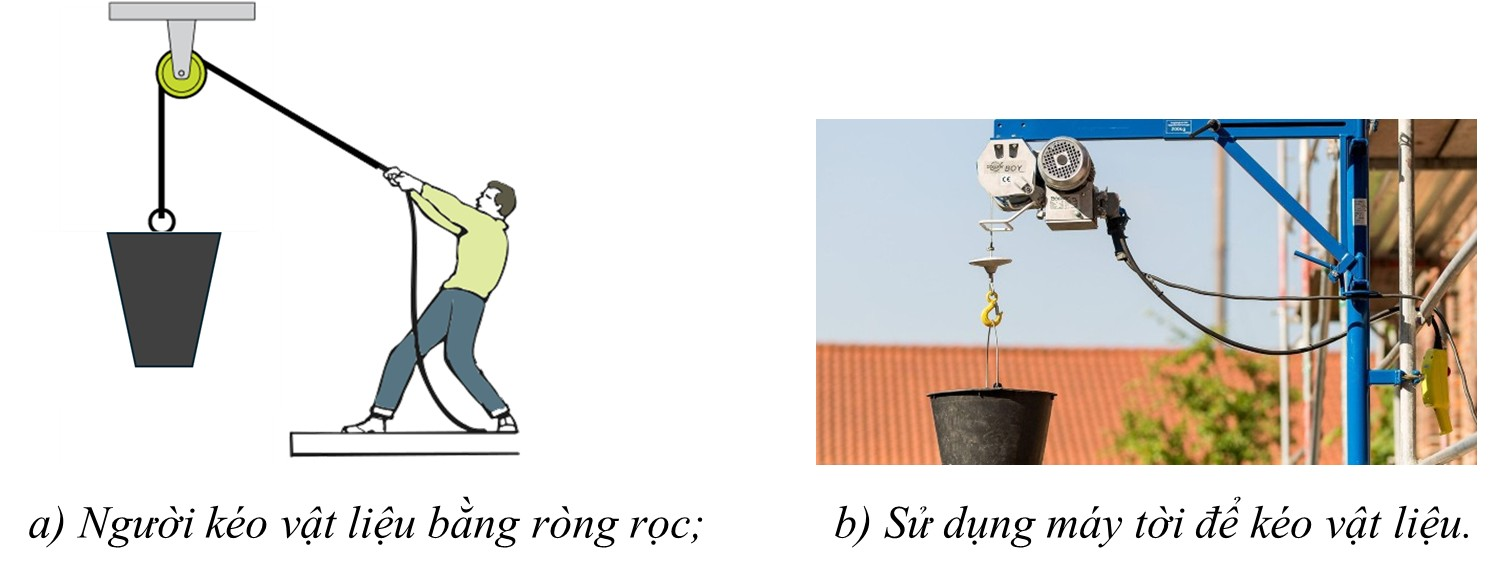
\includegraphics[scale=0.45]{../figs/D10-KTTX2-HK2-1}
	\end{center}
	\choiceTF
	{Khi đưa vật liệu lên cao bằng máy tời điện thì đã có sự chuyển hóa từ cơ năng sang điện năng}
	{\True Công tối thiểu cần thực hiện trong 2 trường hợp như nhau}
	{\True Khi kéo đều khối vật liệu thì công thực hiện của máy tời là \SI{5000}{\joule}}
	{\True Công suất kéo khối vật liệu của người và máy tời lần lượt là \SI{100}{\watt}, \SI{500}{\watt}}
	\loigiai{}
\end{ex}
% ===================================================================
\begin{ex}
	\immini{Một thang máy có khối lượng \SI{1.0E3}{\kilogram} có tải trọng tối đa \SI{8.0E2}{\kilogram}. Lực cản tác dụng lên thang máy không đổi và có độ lớn \SI{4.00E3}{\newton}. Thang máy đang chứa đầy tải trọng và đi lên đều với tốc độ \SI{3.0}{\meter/\second}.
	\choiceTF
	{Trong quá trình thang máy đi lên, trọng lực sinh công dương}
	{\True Độ lớn lực căng của dây cáp tác dụng lên thang máy là \SI{22}{\kilo\newton}}
	{\True Công suất trung bình của thang máy gần \SI{88.5}{HP}}
	{Motor thang máy hoạt động với công suất không đổi, nếu cần tăng độ lớn lực kéo của động cơ thì phải giảm tốc độ chuyển động của thang máy}
	}
	{\vspace{-0.65cm}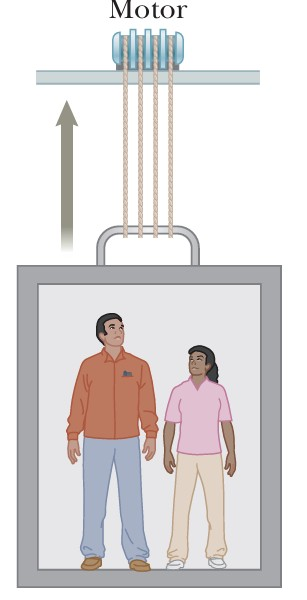
\includegraphics[scale=0.5]{../figs/D10-KTTX2-HK2-2}}
	
	\loigiai{}
\end{ex}
\Closesolutionfile{ans}
\section{Tự luận}
\setcounter{ex}{0}
\Opensolutionfile{ans}[ans/D10-KTTX2-HK2-TL]
% ===============================================================
\begin{ex}
	Nhà máy thủy điện được xây dựng ở những nơi có thác nước cao để lợi dụng năng lượng nước chảy xuống. Tuabin nhà máy phát điện phát ra công suất \SI{25}{\mega\watt}. Biết mỗi phút nước chảy vào tuabin máy phát điện \SI{1800}{\meter^3} và hiệu suất của tuabin là \SI{80}{\percent}. Cho khối lượng riêng của nước là $\rho=\SI{1000}{\kilogram/\meter^3}$. Tính độ cao thác nước theo đơn vị mét $\left(\si{\meter}\right)$ và làm tròn kết quả đến chữ số hàng đơn vị.
	\loigiai{
		
	}
\end{ex}
% ===============================================================
\begin{ex}
	Một vật có khối lượng $m=\SI{10}{\kilogram}$ trượt không vận tốc đầu từ đỉnh của một mặt phẳng nghiêng cao \SI{20}{\meter}. Khi tới chân dốc thì vật có tốc độ \SI{15}{\meter/\second}. Tính công của lực ma sát trong quá trình này theo đơn vị joule $\left(\si{\joule}\right)$.
	\loigiai{
		\SI{-875}{\joule}.
	}
\end{ex}
\Closesolutionfile{ans}